
\begin{figure}[H]
\begin{center}
  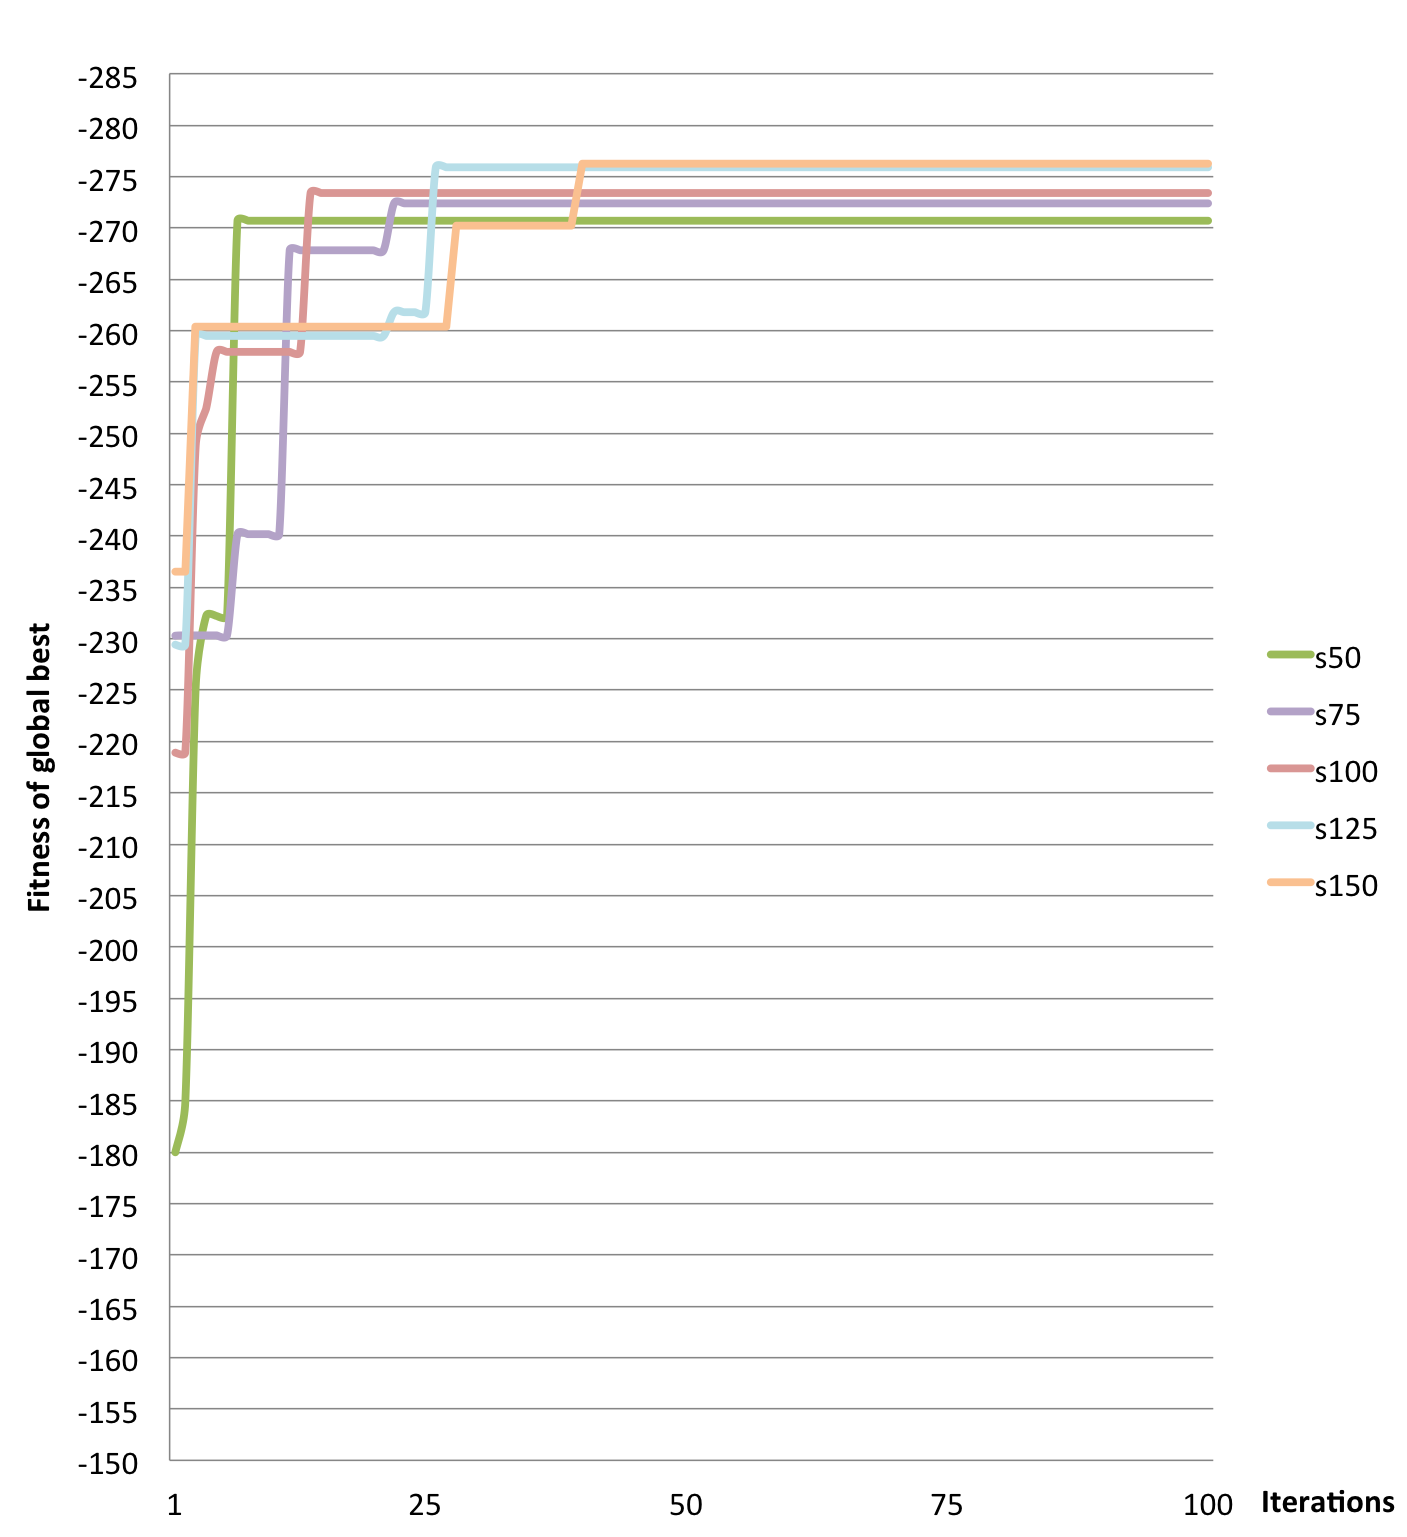
\includegraphics[width=4in]{assets/svsitest.png}
  \end{center}
  \caption{Evaluation of total fitness function when number of iterations in accordance to the colony size($s$) vary}
  \label{fig:svsitesting} 
\end{figure}

\begin{figure}[H]
\begin{center}
  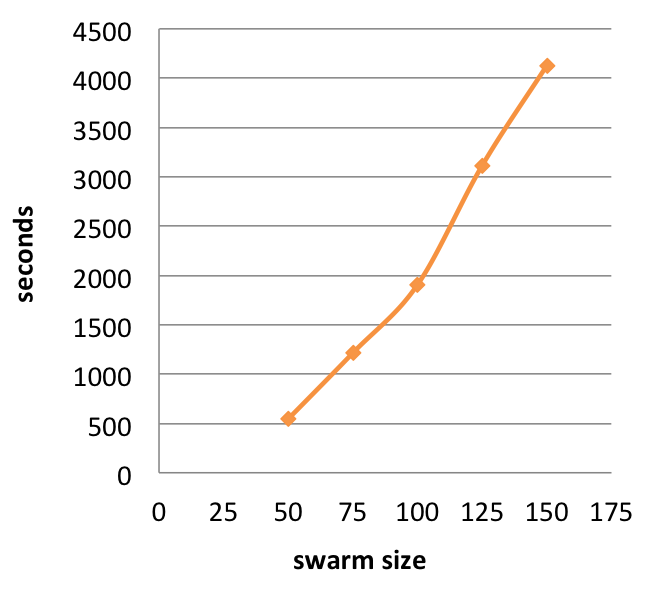
\includegraphics[width=2.5in]{assets/svsiruntime.png}
  \end{center}
  \caption{Evaluation of runtime in accordance to the colony size($s$) \emph{\color{blue} Husk: iterations skal være swarm size}}
  \label{fig:svsiruntime} 
\end{figure}

\textbf{$s$ and $i$ evaluation}
\newline

Figure \vref{fig:svsitesting}, presents the evolution of the fitness function ($TOTFIT$) against the number of ants in the colony, in the case of four routes. The algorithm is run one time for each swarm size, and the fitness value is recorded for each iteration. The first point is the $TOTFIT$ value after the first iteration, where the ants are starting its tour with a clean state.

As one can see, increasing the size of the colony leads to a better $TOTFIT$ value in both the initial and final iterations. 

One can observe that the $TOTFIT$

After increasing the the colony the $totfit$ appears to converge a little later. If we use a small colony size it is possible that the search will be trapped in a local optima, given the small diversity in the initial population.  

 The total fitness function (TOTFIT), decreases faster in the early iterations, when the number of the colony size decreases. But when the number of iterations reaches 30 to 40 iterations, 